\documentclass{ceurart}

\usepackage{acronym}
\usepackage{subcaption}
\usepackage{tikz}
\usetikzlibrary{positioning}
\usepackage{threeparttable}

\renewcommand{\acffont}[1]{\textsl{#1}}


%%
%% end of the preamble, start of the body of the document source.
\begin{document}

%%
%% Rights management information.
%% CC-BY is default license.
\copyrightyear{2025}
\copyrightclause{Copyright for this paper by its authors.\\
  Use permitted under Creative Commons License Attribution 4.0
  International (CC BY 4.0).}

%%
%% This command is for the conference information
\conference{``Search Engines'', course at the master degree in ``Computer Engineering'', Department of Information Engineering, and at the master degree in ``Data Science'', Department of Mathematics ``Tullio Levi-Civita'', University of Padua, Italy. Academic Year 2024/2025}

%%
%% The "title" command
\title{SEUPD@CLEF: Team Searchill}

%%
%% The "author" command and its associated commands are used to define
%% the authors and their affiliations.
\author[1]{Alessandro Di Frenna}[%
email=Alessandro.DiFrenna@studenti.unipd.it
]

\author[1]{Andrea Di Tillo}[%
email=Andrea.DiTillo@studenti.unipd.it
]

\author[1]{Luca Pellegrini}[%
email=Luca.Pellegrini@studenti.unipd.it
]

\author[1]{Marco Tomaiuoli}[%
email=Marco.Tomaiuoli@studenti.unipd.it
]

\author[1]{Artur Voit-Antal}[%
email=Artur.VoitAntal@studenti.unipd.it
]

\address[1]{University of Padua, Italy}


%%
%% The abstract is a short summary of the work to be presented in the
%% article.
\begin{abstract}
  This report describes the search engine developed by the team "Searchill" for the LongEval-Retrieval Task 1 at the CLEF 2025 conference. The main objective of the project was to develop an effective yet efficient search engine. To achieve this goal, our team has extensively experimented with various techniques and approaches. To assess system performance, we used the CLEF corpus and human judgements. 
  Our top-performing system, which combines traditional methods with AI, has encouraging results and might be the basis for further advancements in the field.
\end{abstract}

%%
%% Keywords. The author(s) should pick words that accurately describe
%% the work being presented. Separate the keywords with commas.
\begin{keywords}
  CLEF 2023 \sep
  LongEval \sep
  Information Retrieval \sep
  Search Engine \sep
  Natural Language Processing  
\end{keywords}

%%
%% This command processes the author and affiliation and title
%% information and builds the first part of the formatted document.
\maketitle


\section{Introduction}
\label{sec:introduction}

The amount of information available online has been rapidly increasing due to the internet's fast growth, making it difficult to find reliable and pertinent information. Search engines are essential in this situation as they allow users to quickly and easily locate accurate information. Information retrieval systems are now essential in almost all the fields. Our study investigates the complexities of information retrieval and how it can be enhanced, as well as how well they can adjust to the changing digital environment. 

The goal of this research is to create a reliable retrieval system that can handle the ever-changing nature of the internet. We do this by using the Longeval Websearch collection \cite{longeval2025}, an extensive dataset of online pages, topics, and user interactions. As a result of this effort, our understanding of information retrieval systems in the context of search engines has greatly improved. In particular, we focused on improving query and document processing methods to maximise ranking outcomes and provide users with the most relevant information.

The paper is organized as follows: Section~\ref{sec:methodology} describes our approach; Section~\ref{sec:setup} explains our experimental setup; Section~\ref{sec:results} discusses our main findings; finally, Section~\ref{sec:conclusion} draws some conclusions and outlooks for future work.

\subsection{Related Work}
To begin addressing the project requirements, we conducted a thorough analysis of the specifications and file formats necessary for implementation. We relied on materials provided by the CLEF LongEval \cite{longeval2025} website and the accompanying 2023 documentation \cite{alkhalifa2023clef} to identify the essential elements needed to organize our workflow effectively. Guided by the tutoring sessions from the SearchEngines course at the University of Padua, we proceeded with the development of the key components—indexer, analyzer, and searcher—following the framework introduced and discussed in class. For implementing the re-ranker, we employed the API offered and documented by Cohere \cite{cohereAbout2025}.

\section{Methodology}
\label{sec:methodology}

In this section, we describe the methodology adopted to develop our IR system for the task.


\subsection{Parser}
The parser is responsible for reading and extracting structured data from complex document formats, enabling effective indexing and retrieval. Our document parsing framework consists of several components designed to handle different document structures efficiently:

\begin{itemize}

\item \textbf{DocumentParser:} This abstract class serves as the core of our parsing framework. It provides a template for iterating over documents. The class ensures that documents are read correctly.

\item \textbf{ParsedDocument:} This class encapsulates the structure of a parsed document. It defines essential fields such as:
  \begin{itemize}
    \item \texttt{ID} - A unique identifier for each document.
    \item \texttt{Body} - The main content of the document.
    \item \texttt{Start} - Initial lines of the document, often used for quick reference.
    \item \texttt{Highlights} - Notable words or phrases extracted from tags or special formatting, enhancing keyword extraction.
  \end{itemize}

\item \textbf{TrecParser:} This specialized class extends \texttt{DocumentParser} to handle TREC-formatted documents. Key functions include:
  \begin{itemize}
    \item Regex-based extraction of document fields such as \texttt{<DOCNO>} and \texttt{<DOCID>}.
    \item Management of document content using a multistage buffering approach to efficiently handle large text bodies.
    \item Extraction of emphasized content through patterns such as \texttt{hashtags} and \texttt{strong} tags, improving the semantic richness of stored highlights.
    \item Support for emoji and URL filtering, ensuring text data is clean and normalized before analysis.
  \end{itemize}

\item \textbf{Error Handling:} Robust error management is implemented to gracefully handle missing or malformed data, maintaining the stability and reliability of the parser.

\end{itemize}

This structured parsing methodology allows for the seamless transformation of raw text into well-defined data objects, paving the way for accurate indexing and retrieval operations.



\subsection{Analyzer}
The \texttt{FrenchAnalyzer} is designed to process French texts, integrating multiple components to ensure accurate analysis:

\begin{itemize}
    \item \textbf{Tokenization:} We provide multiple tokenizer options to cater to different text handling needs:
    \begin{itemize}
        \item \texttt{WhitespaceTokenizer} - Splits texts at whitespace, ideal for structured input.
        \item \texttt{LetterTokenizer} - Separates tokens at non-letter characters, useful for handling alphabetic text.
        \item \texttt{StandardTokenizer} - Uses advanced parsing rules for handling more complex textual structures, such as handling punctuation and special characters. Includes Named Entity Recognition (NER) for recognising email addresses, URLs, and numeric sequences as single tokens. 
        \item \texttt{OpenNLPTokenizer} - Uses OpenNLP statistical models for tokenization, which is beneficial for handling complex language.
    \end{itemize}

    \item \textbf{Character Folding:} Using \texttt{ICUFoldingFilter}, characters are normalized to their basic forms, standardizing variations such as accented characters to their base, which improves the uniformity of the processing.

    \item \textbf{Elision Removal:} The \texttt{ElisionFilter} targets contracted French words, removing apostrophes and similar contractions, treating contractions like "l'histoire" simply as "histoire".

    \item \textbf{Abbreviation Expansion:} The \texttt{AbbreviationExpansionFilter} employs a predefined map to expand abbreviations, ensuring that terms such as "Dr." are expanded to "Doctor", further improving processing uniformity.

    \item \textbf{POS Tagging and Compound Formation:} Through \texttt{CompoundPOSTokenFilter}, part-of-speech tags are assigned using the OpenNLP POS model. This allows for recognising compound words as such and treating them as single tokens.

    \item \textbf{N-grams Generation:} \texttt{ShingleFilter} is optionally applied to produce n-grams that capture context within a specified window size. 

    \item \textbf{Stopword Removal:} The \texttt{StopFilter}, loaded with a list of irrelevant tokens, removes common stopwords that do not contribute to the semantic meaning of texts and queries.

    \item \textbf{Length Filtering:} The \texttt{LengthFilter} ensures that only tokens within a specified character range are retained, filtering out noise and exceedingly frequent short tokens.

    \item \textbf{Position Increment Adjustment:} Implemented via \texttt{PositionFilter}, this adjusts the \texttt{positionIncrement} attribute of tokens, maintaining consistent positional data for proximity-based queries.

    \item \textbf{Stemming and Lemmatization:} customised to handle French morphology:
    \begin{itemize}
        \item \texttt{FrenchLightStemFilter} - Applies a light stem, suitable for texts requiring minimal conversion.
        \item \texttt{FrenchMinimalStemFilter} - Executes minimal stemming, avoiding over-reduction.
        \item \texttt{SnowballFilter}(snow) - Employs the Snowball stemming algorithm, recognized for its effectiveness across languages.
        \item \texttt{OpenNLPLemmatizerFilter} - A lemmatization approach that uses OpenNLP to convert words to their base forms, capturing the underlying semantics.
    \end{itemize}
\end{itemize}

\begin{center}
    \begin{figure}[h]
        \centering
        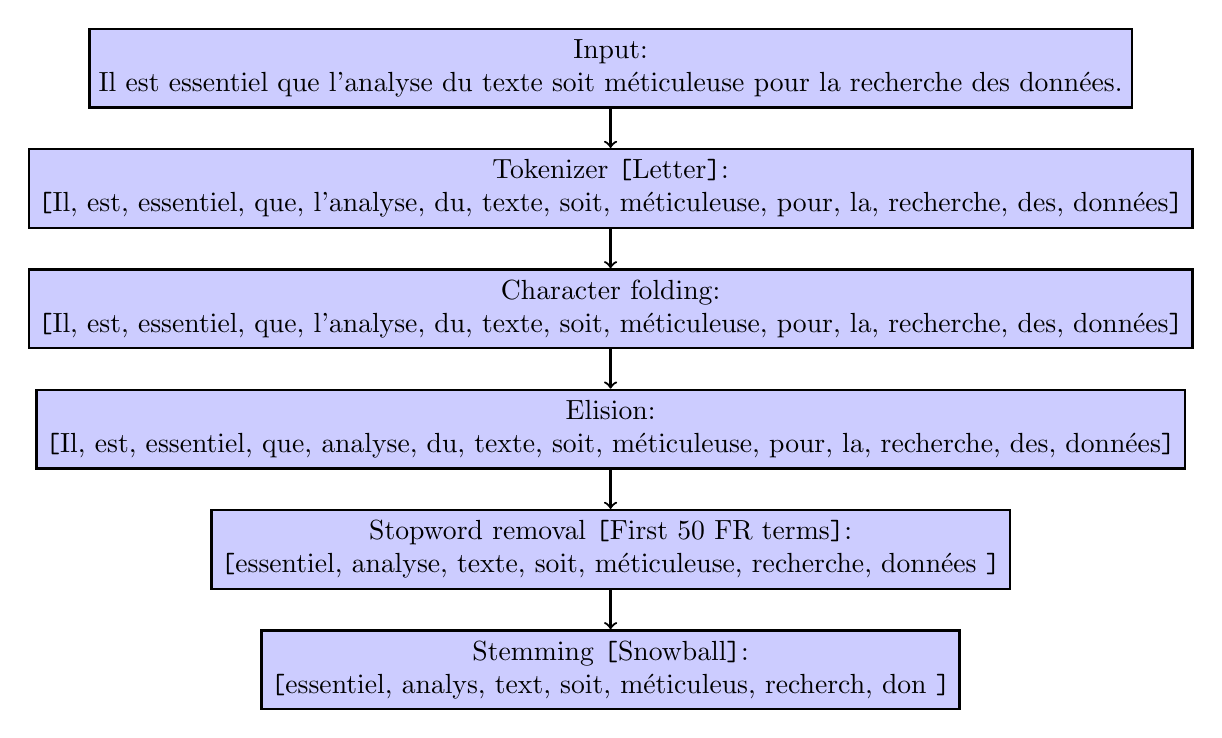
\begin{tikzpicture}[node distance=0.5cm and 0.5cm, auto]
            % Nodes
            \node[rectangle, draw, thick, align=center, fill=blue!20, minimum width=3cm, minimum height=1cm] (stage1) {Input:
            \\ Il est essentiel que l'analyse du texte soit méticuleuse pour la recherche des données.};

            \node[rectangle, draw, thick, align=center, fill=blue!20, minimum width=3cm, minimum height=1cm, below=of stage1] (stage2) {Tokenizer \texttt{[}Letter\texttt{]}:
            \\
            \texttt{[}Il, est, essentiel, que, l'analyse, du, texte, soit, méticuleuse, pour, la, recherche, des, données\texttt{]}};

            \node[rectangle, draw, thick, align=center, fill=blue!20, minimum width=3cm, minimum height=1cm, below=of stage2] (stage3) {Character folding:
            \\
            \texttt{[}Il, est, essentiel, que, l'analyse, du, texte, soit, méticuleuse, pour, la, recherche, des, données\texttt{]}};

            \node[rectangle, draw, thick, align=center, fill=blue!20, minimum width=3cm, minimum height=1cm, below=of stage3] (stage4) {Elision:
            \\
            \texttt{[}Il, est, essentiel, que, analyse, du, texte, soit, méticuleuse, pour, la, recherche, des, données\texttt{]}};

            \node[rectangle, draw, thick, align=center, align=center, fill=blue!20, minimum width=3cm, minimum height=1cm, below=of stage4] (stage5) {Stopword removal \texttt{[}First 50 FR terms\texttt{]}:
            \\
            \texttt{[}essentiel, analyse, texte, soit, méticuleuse, recherche, données \texttt{]}
            };

            \node[rectangle, draw, thick, align=center, align=center,fill=blue!20, minimum width=3cm, minimum height=1cm, below=of stage5] (stage6) {Stemming \texttt{[}Snowball\texttt{]}:
            \\
            \texttt{[}essentiel, analys, text, soit, méticuleus, recherch, don \texttt{]}
            };

            \draw[->, thick] (stage1) -- (stage2);
            \draw[->, thick] (stage2) -- (stage3);
            \draw[->, thick] (stage3) -- (stage4);
            \draw[->, thick] (stage4) -- (stage5);
            \draw[->, thick] (stage5) -- (stage6);
        \end{tikzpicture}
        \caption{Example of the analyzer process.}
        \label{fig:fr_analyzer_process}
    \end{figure}
\end{center}

\newpage
\subsection{Indexer}

\begin{itemize}
    \item \textbf{BodyField}: \begin{itemize}
                                  \item \textbf{BodyField}: represents the body field of a document: \begin{itemize}
                                                                                                         \item \textbf{token}: the body is broken into tokens.
                                                                                                         \item \textbf{frequency}: we save the frequency of the tokens.
                                                                                                         \item \textbf{position}:  we save the position of the tokens, this allows us to use phrase queries.
                                                                                                         \item \textbf{body store}: we save the body of the documents, this allows us to pass the document's bodies to a re-ranker.

                                  \end{itemize}
                                  \item \textbf{StartField}: \begin{itemize}
                                                                 \item \textbf{token}: the start is broken into tokens.
                                                                 \item \textbf{frequency}: we save the frequency of the tokens.
                                                                 \item \textbf{body store}: we save the start of the documents.
                                  \end{itemize}
                                  \item \textbf{HighlightedField}: \begin{itemize}
                                                                 \item \textbf{token}: the hightlighted is broken into tokens.
                                                                 \item \textbf{frequency}: we save the frequency of the tokens.
                                                                 \item \textbf{body store}: we save the highlights of the documents.
                                  \end{itemize}
    \end{itemize}
    \item \textbf{DirectoryIndexer}: \newline
    \setlength\parindent{24pt} This class indexes documents found within a designated directory. It allows for several parameters, such as the directory where the documents are stored, the type of parser used to parse the documents, the analyzer used to process the text, the similarity metric employed for indexing, the anticipated number of documents, and the location where the resulting index will be saved.

        \begin{center}
        \begin{table}[h]
            \centering
            \begin{tabular}{|c|c|c|c|c|}
                \hline
                Collection & Docs Size (GB) & Body Terms & Number of Documents & Index Size (GB) \\
                \hline
                French 2022-06 & 9,3 & 3,423,470 & 1,590,024 & 7.5 \\
                \hline
                French 2023-01 & 12.8 & 38,313,777 & 2,537,554 & 12.4 \\
                \hline
            \end{tabular}
            \caption{Indexing output details.}
            \label{tab:Indexing_details}
        \end{table}
    \end{center}

\end{itemize}

\subsubsection{StopList Choice}
After we have indexed all the documents part of the training set, we used LUKE, a tool provided by Lucene that allowed us to inspect our indexed documents and see how the documents were indexed and identify the most frequent tokens in our collection.
\\ \\
After indexing all the French documents without using stop lists or Stemmers, we observed the first lines of results.

\begin{flushleft}
    We noticed there are English terms and numbers with significant frequency values alongside French terms. Based on this observation, we decided to create various stop lists incorporating different combinations of numbers, English terms, or both. We then examined the computational results of these configurations. All this was done to verify the importance that these elements have in the context of the documents analyzed.
\newline
    The created stop lists are:
    \begin{itemize}
        
        \item \textbf{stopList40FR-10EN :} It contains the first 40 French terms and 10 English terms.

        \item \textbf{stopList40FR-10NUM :} It contains the first 40 French terms and 10 numbers.

        \item \textbf{stopList35FR-10EN-5NUM :} It contains the first 35 French terms, 10 english words and 5 numbers.

        \item \textbf{stopList50FR-2022-06 :} It contains the first 50 French terms from the French collection 2022-06.
        
        \item \textbf{stopList50FR-2023-01 :} It contains the first 50 French terms from the French collection 2023-01.
    \end{itemize}
\end{flushleft}

We chose the best one, and decided to use it for all the runs.
\begin{itemize}
    \item  \textbf{Stoplists tuning:}
\end{itemize}

\begin{table}[ht]
    \centering
    \begin{minipage}{0.48\textwidth}
        \centering
        \begin{tabular}{ |l|c|c| }
            \hline
            Run name 2022-06 & nDCG & MAP \\
            \hline\hline
            stoplist-BstoplistFR & 0,1682 & 0.0896 \\
            stoplist-50FR & 0,1681 & 0.0897 \\
            stoplist-40FR-10N & 0,1673 & 0.0890 \\
            \rowcolor{LightYellow}
            stoplist-40FR-10EN & 0,1694 & 0.0902 \\
            stoplist-35FR-10EN-5N & 0,1679 & 0.0894 \\
            \hline
        \end{tabular}
        \caption{Stoplist tuning table 2022-06.}
        \label{tab:stoplist-2022}
    \end{minipage}
    \hfill
    \begin{minipage}{0.48\textwidth}
        \centering
        \begin{tabular}{ |l|c|c| }
            \hline
            Run name 2023-01 & nDCG & MAP \\
            \hline\hline
            stoplist-BstoplistFR & 0,2540 & 0.1620 \\
            stoplist-50FR & 0,2545 & 0.1624 \\
            stoplist-40FR-10N & 0,2530 & 0.1619 \\
            \rowcolor{LightYellow}
            stoplist-40FR-10EN & 0,2587 & 0.1631 \\
            stoplist-35FR-10EN-5N & 0,2531 & 0.1622 \\
            \hline
        \end{tabular}
        \caption{Stoplist tuning table 2023-01.}
        \label{tab:stoplist-2023}
    \end{minipage}
\end{table}

\begin{itemize}
    \item  \textbf{Stemmer tuning:}
\end{itemize}

\begin{table}[ht]
    \centering
    \begin{minipage}{0.48\textwidth}
        \centering
        \begin{tabular}{ |l|c|c| }
            \hline
            Run name 2022-06 & nDCG & MAP \\ [0.5ex]
            \hline\hline
            stem-FrenchLight & 0.1398 & 0.0703 \\
            \rowcolor{LightYellow}
            stem-SnowBall & 0.1499 & 0.0767 \\
            stem-FrenchMinimal & 0.1426 & 0.0722 \\
            \hline
        \end{tabular}
        \caption{Stemmer tuning 2022-06}
        \label{tab:stemmer-a}
    \end{minipage}
    \hfill
    \begin{minipage}{0.48\textwidth}
        \centering
        \begin{tabular}{ |l|c|c| }
            \hline
            Run name 2023-01 & nDCG & MAP \\ [0.5ex]
            \hline\hline
            stem-FrenchLight & 0.2207 & 0.1345 \\
            \rowcolor{LightYellow}
            stem-SnowBall & 0.2315 & 0.1422 \\
            stem-FrenchMinimal & 0.2250 & 0.1370 \\
            \hline
        \end{tabular}
        \caption{Stemmer tuning 2023-01}
        \label{tab:stemmer-b}
    \end{minipage}
\end{table}

\begin{itemize}
    \item  \textbf{Tokenizer tuning:}
\end{itemize}

\begin{table}[ht]
    \centering
    \begin{minipage}{0.48\textwidth}
        \centering
        \begin{tabular}{ |l|c|c| }
            \hline
            Run name 2022-06 & nDCG & MAP \\ [0.5ex]
            \hline\hline
            tokenizer-WhiteSpace & 0.1541 & 0.0796 \\
            \rowcolor{LightYellow}
            tokenizer-Letter & 0.1723 & 0.0923 \\
            tokenizer-Standard & 0.1710 & 0.0919 \\
            \hline
        \end{tabular}
        \caption{Stemmer tuning 2022-06}
        \label{tab:stemmer-a}
    \end{minipage}
    \hfill
    \begin{minipage}{0.48\textwidth}
        \centering
        \begin{tabular}{ |l|c|c| }
            \hline
            Run name 2023-01 & nDCG & MAP \\ [0.5ex]
            \hline\hline
            tokenizer-WhiteSpace & 0.2420 & 0.1512 \\
            \rowcolor{LightYellow}
            tokenizer-Letter & 0.2675 & 0.1710 \\
            tokenizer-Standard & 0.2656 & 0.1695 \\
            \hline
        \end{tabular}
        \caption{Stemmer tuning 2023-01}
        \label{tab:stemmer-b}
    \end{minipage}
\end{table}


\subsection{Searcher}
\label{subsec:searcher}
Within the searcher component, a Boolean query strategy was employed to facilitate query expansion and enhance the overall effectiveness of the information retrieval system. The initial query terms were designated as mandatory for document retrieval, while the expanded terms were incorporated as optional elements, thereby allowing for greater flexibility in matching relevant documents. Furthermore, a boosting mechanism was applied to assign increased weight to the original query, reinforcing its central role in the retrieval process. The subsequent section provides a detailed account of the query expansion methodology implemented.

\subsubsection{Start}
\label{subsubsec:Start}
It is commonly observed that the core subject matter of a document is often introduced at the beginning of the text. Building upon this assumption, we implemented a strategy within the indexer to store the first five lines of each document, leveraging the structural layout provided by the LongEval dataset in TREC format. This design choice allowed the search engine to perform query operations specifically within this initial segment — termed the \texttt{start} — rather than scanning the entire document body.

To further enhance retrieval precision, we assigned greater weight to query matches occurring within the \texttt{start} section compared to those found elsewhere in the document. The underlying rationale was that documents introducing the query terms early on are more likely to align with the user's search intent. This emphasis on the initial portion was intended to improve both the relevance and the overall quality of the retrieved results.

\subsubsection{N-grams}
\label{subsubsec:Start}
As an initial step in our query expansion strategy, we employed word N-grams—sequences of adjacent terms extracted from the original query—to enrich the query representation. This process involves tokenizing the original query into individual words and subsequently recombining them into contiguous word pairs. For example, the query "\texttt{running shoes women}" is tokenized into "\texttt{running}", "\texttt{shoes}", and "\texttt{women}", from which we generate the bi-grams "\texttt{running shoes}" and "\texttt{shoes women}".

While this technique has the potential to enhance retrieval accuracy by capturing meaningful term associations, we deliberately assigned a lower weight to these expanded terms within the Boolean query formulation. This decision was made to prioritize documents that more closely align with the original query, thus preserving its semantic integrity.

Moreover, we restricted the generation of N-grams to a maximum of two words. In our view, extending the N-gram length beyond this threshold would introduce an excessive number of query variants, potentially diluting the relevance of the results and increasing computational overhead.


\subsubsection{Fuzzy Search}
\label{subsubsec:fuzzy}
To further improve the robustness of our search system, we integrated a fuzzy search mechanism capable of handling approximate matches between query terms and document content. This technique is particularly effective in addressing minor input errors such as typographical mistakes, letter transpositions, or common abbreviations. By setting a similarity threshold, the system ensures that only plausible variations of the query terms are considered, thereby maintaining an acceptable level of accuracy. For example, a query such as "\texttt{Adibas chaussures}" may successfully retrieve documents containing the correctly spelled brand name "\texttt{Adidas}".

The fuzzy searcher leverages the Damerau–Levenshtein distance as its core similarity metric. This algorithm—also referred to as the optimal string alignment distance—quantifies the dissimilarity between two strings based on the minimum number of edit operations (insertions, deletions, substitutions, or adjacent transpositions) required to transform one string into the other.

In our implementation of fuzzy search \cite{luceneFuzzyQuery2024}, candidate terms are collected and scored according to their respective edit distances, with only the highest-ranking terms incorporated into the expanded query. Importantly, we deliberately avoided using high distance thresholds, as such configurations tend to generate overly broad matches, ultimately reducing retrieval precision and degrading overall system performance.
\vspace{\baselineskip}

\textbf{Fuzzy Tuning}

To assess the effectiveness of incorporating fuzzy queries within our Boolean query framework, we employed an empirical evaluation strategy. Specifically, we compared the performance of a baseline configuration — where no query expansion techniques were applied and only the original query was used — against a series of runs integrating fuzzy queries with varying weight parameters. This process, which we refer to as \texttt{Fuzzy Tuning}, aimed to isolate and measure the contribution of fuzzy matching to retrieval performance. Notably, all experiments were conducted without the use of the re-ranking component.

\vspace{\baselineskip}

We determined that a weight increment of 0.1 constituted a suitable compromise between granularity and experimental feasibility, as finer increments (e.g., 0.05) would have necessitated a disproportionately high number of runs without a commensurate gain in insight.

\vspace{\baselineskip}

As illustrated in Table 5, the optimal performance was observed when the fuzzy component was assigned a weight of 0.1. This result is consistent with the intended role of fuzzy filtering: while it is effective at capturing minor orthographic variations (e.g., typographical errors or alternate spellings), overemphasizing its contribution may inadvertently amplify terms that are lexically similar yet semantically unrelated. Consequently, excessive weighting can degrade the quality of the retrieved documents by introducing noise into the results.

\subsubsection{Dictionary}
\label{subsubsec:Dictionary}
During the analysis of user input, we observed that certain queries appeared in unconventional formats, such as URLs, dot-separated terms (e.g., \texttt{term1.term2.term3}), or concatenated words without spacing (e.g., \texttt{term1term2term3}), which posed challenges for effective processing by the search engine. To mitigate issues caused by punctuation, we implemented a function based on regular expressions to systematically remove such characters from the input.

In addressing the problem of concatenated terms, we employed a dictionary derived from the provided synonyms file. This dictionary enables the system to identify and extract meaningful sub-terms embedded within single-word queries. Notably, this approach was applied exclusively to queries composed of a single token, as extending it to multi-word queries introduced considerable computational overhead and negatively impacted system performance.

The motivation for focusing on single-word queries lies in the higher likelihood of such inputs being affected by typographical errors. In these cases, suggesting alternative or similar terms can significantly enhance retrieval quality. Conversely, in multi-word queries, the probability of all constituent terms being misspelled is low; thus, attempting to alter each term could reduce both precision and overall system effectiveness.

\subsubsection{Synonyms}
\label{subsubsec:synonyms}
Implementing synonyms in retrieval poses challenges, including semantic ambiguity and noise due to polysemy and irrelevant matches. While synonyms theoretically broaden search scope, actual gains depend on context-specific relevance. To mitigate computational overhead, synonyms were managed at query time using a query expansion model. This approach aims to enhance retrieval accuracy while maintaining system efficiency.

Consider the example query "\texttt{Chat orange}", normally, the information retrieval (IR) system first parses and analyzes the query and searches for "\texttt{orange}" and "\texttt{chat}". However, if a relevant document contains "\texttt{gingembre}" instead of "\texttt{orange}" and "\texttt{félin}" instead of "\texttt{chat}", the document will not be considered relevant. The searcher takes the original query, searches a synonym collection for synonyms of those words, and retrieves three synonyms. If there are more than three available in the collection, three synonyms are chosen randomly, and these are then added to the Boolean query. We chose to use a synonym collection sourced from GitHub \cite{lorenzon2016vim}. 

\textbf{Synonyms Tuning}: Since the synonyms approach involves selecting three random synonyms from the collection, we chose not to adopt an experimental approach as we did with the Fuzzy and Phrase tools, due to a lack of repeatability stemming from the aforementioned randomness. We assigned a weight of 0.1 to each synonym to maintain the choices made for the Phrase and Fuzzy Query tools.

\subsubsection{Phrase Query}
\label{subsubsec: Phrase Query }

To further enhance the precision of our retrieval system, we implemented a \textbf{Phrase Query Searcher} designed to identify documents containing a specific sequence of terms in the exact or near-exact order in which they appear in the query. Phrase queries require that the specified terms occur in contiguous positions within the document. However, to allow for a degree of flexibility in term positioning, we employed the \textit{slop} parameter, which defines the maximum number of positional shifts permitted between the terms.

This mechanism is particularly beneficial in accommodating natural variations in language, such as minor rearrangements or the insertion of additional words. For example, a query for the phrase ``quick brown fox'' with a slop value of $1$ would also match documents containing ``quick fox brown,'' thereby increasing recall without significantly deviating from the original query intent.

The incorporation of phrase queries thus improves the search engine’s ability to retrieve documents that closely align with the semantic structure of the user input, even when exact word order is not preserved.

In the context of LongEval 2025 \cite{longeval2025} the official queries are provided in two formats. The first follows the TREC format, structured as:

\begin{verbatim}
<top>
<num>q062228</num>
<title>aeroport bordeaux</title>
</top>
\end{verbatim}

Here, the \texttt{<num>} tag denotes the query identifier, while the \texttt{<title>} tag contains the textual content of the query~\cite{reference5}. The alternative format, a TSV (tab-separated values) representation, is structured as:

\begin{verbatim}
62228 aeroport Bordeaux
\end{verbatim}

In this case, the query identifier and the query text are separated by whitespace \cite{longeval2025readme}.

\subsubsection{Word2Vec}
\label{subsubsec: Word2Vec}
To provide word similarity functionality through a web-accessible interface, we developed a lightweight HTTP server using the Flask framework, chosen for its simplicity and ease of deployment in small-scale applications. At the core of the system lies the \texttt{KeyedVectors} interface from the Gensim library, which allows efficient loading and querying of pre-trained word embedding models.

For our implementation, we employed the 300-dimensional French fastText word vectors (cc.fr.300.vec), which were trained on a large-scale Common Crawl corpus. These vectors are particularly suitable for capturing semantic relationships between words in French, thanks to their subword-based architecture that improves coverage and performance on rare or morphologically rich terms.

The application exposes a single RESTful endpoint, \texttt{/similar}, designed to handle HTTP GET requests. Clients can query this endpoint by passing a word as a query parameter. To ensure consistent and reliable behavior, especially in the face of spelling variants and orthographic inconsistencies, the input word is first normalized: it is converted to lowercase and stripped of any diacritics using the unidecode library. This preprocessing step helps enhance the robustness of the similarity computation, enabling more tolerant matching and improved usability in real-world scenarios.

The main purpose of this service is to support query expansion within our information retrieval pipeline. When a user submits a search query, the system sends the main term to the \texttt{/similar} endpoint. The endpoint responds with a list of semantically related words retrieved from the fastText embeddings. These similar terms are then automatically appended to the original query, effectively expanding it. This strategy enhances recall by allowing the retrieval system to consider contextually related terms, improving the chances of retrieving relevant documents even when exact matches are not present.


\subsubsection{LLM}
\label{subsubsec:LLM}
LLM-based query expansion is a technique used to enhance the effectiveness of a search engine by automatically expanding the original query formulated by the user. This methodology is particularly useful in cases where the user input is too generic, vague, or ambiguous, and therefore insufficient to return truly relevant results.

In our case, the query is sent to a Large Language Model (LLM), specifically \textit{ChatGPT-3.5-turbo}, which is responsible for interpreting the meaning of the sentence and generating three to four related terms.

This number of terms was chosen strategically: an expansion that is too broad would introduce informational noise, potentially reducing the precision of the results, while an expansion that is too narrow would compromise the overall effectiveness of the technique.

We therefore opted for a balanced solution, capable of enriching the query in a meaningful yet controlled way. These terms are not simple synonyms, but semantically related concepts that help enrich the context of the search. The goal is to provide the search engine with additional cues to identify relevant documents, even when they do not contain the exact terms used in the original query.

The choice of using ChatGPT-3.5-turbo was driven by a trade-off between performance and cost: although less powerful and accurate than more advanced models such as GPT-4o or GPT-4.1, it proved to be sufficiently effective for our needs, at a significantly lower price compared to its counterpart.



\subsubsection{Query Construction}
\label{subsubsec:Query Construction}
The core search process employs a dynamic Boolean query builder with weighted clauses:

\begin{itemize}
    \item \textbf{Base Query}: Mandatory clause parsed from the original query string
    \item \textbf{Field Boosting}:
    \begin{itemize}
        \item Start field matches boosted by 1.5$\times$
        \item Highlight field matches boosted by 1.2$\times$
    \end{itemize}
    \item \textbf{Query Expansion}: Optional features:
    \begin{itemize}
        \item Dictionary-based synonyms (0.1$\times$ weight)
        \item Fuzzy search with edit distance=2 (0.2$\times$-0.8$\times$ weights), which allows for typos
        \item Phrase queries with slop=5 window
    \end{itemize}
\end{itemize}

\subsubsection{Query Expansion Techniques}
\label{subsubsec:Query Expansion Techniques}
We implemented six complementary expansion strategies:

\paragraph{N-grams Generation}
\begin{itemize}
    \item Uses ShingleFilter with default 2-gram window
    \item Applies 0.3$\times$ weight to generated bigrams
    \item Filters single-word n-grams post-generation
\end{itemize}

\paragraph{Synonym Expansion}
\begin{itemize}
    \item Loads synonym mappings
    \item Distributes weights equally among synonyms
    \item Randomly selects 3 synonyms per term when multiple exist
\end{itemize}

\paragraph{Neural Expansion}
\begin{itemize}
    \item LLM-based term generation via GPT-3.5/DeepSeek APIs
    \item Requests 5-10 related terms per query
    \item Applies 0.4$\times$ weight to generated terms
\end{itemize}

\paragraph{Pseudo-Relevance Feedback (PRF)}
\begin{itemize}
    \item Extracts top 20 terms from initial results
    \item Re-searches with expanded 0.5$\times$ weighted terms
    \item Filters short tokens (<3 characters)
\end{itemize}

\subsubsection{Re-ranking Pipeline}
\label{subsubsec:Re-ranking Pipeline}
Final results undergo neural re-ranking:

\begin{enumerate}
    \item Normalize initial scores to [0,1] range
    \item Retrieve top 100 document bodies
    \item Invoke Cohere multilingual-v3 re-ranker
    \item Combine scores using linear interpolation:
    \[
    \mathit{finalScore} = 0.4 \cdot \mathit{BM25} + 0.6 \cdot \mathit{CohereScore}
    \]
\end{enumerate}

\subsubsection{BM25}
\label{subsubsec:BM25}
For document scoring, we adopted the \textbf{BM25} ranking algorithm \cite{robertson2009bm25}, a well-established probabilistic retrieval model known for its effectiveness in information retrieval tasks. BM25 evaluates the relevance of documents based on term frequency, inverse document frequency, and document length normalization.

A notable limitation of BM25 lies in its sensitivity to parameter tuning, as identifying the optimal values for its parameters (typically $k_1$ and $b$) can be a non-trivial task. To address this, we opted to employ the default parameter settings provided by the Lucene library. This choice was guided by the consideration that manual parameter optimization might lead to overfitting on the development dataset, thereby impairing the model's generalization capability on previously unseen data.


\section{Experimental Setup}
\label{sec:setup}

The experiments were conducted on a MacBook M1 Pro with the following hardware specifications:
\begin{itemize}
    \item \textbf{CPU:} Apple Silicon M1 Pro, 8-core
    \item \textbf{GPU:} Integrated Apple Silicon M1 Pro, 14-core
    \item \textbf{RAM:} 16 GB LPDDR5, 3200 MHz
    \item \textbf{Storage:} 512 GB SSD with sequential read speeds of up to 4,900 MB/s and write speeds of up to 3,951 MB/s
\end{itemize}

The datasets utilized in this study are those made available by the LongEval CLEF 2025 Lab, accessible at: \href{https://clef-longeval.github.io/data/}{https://clef-longeval.github.io/data/}

The full implementation of the project can be found at: \href{https://bitbucket.org/upd-dei-stud-prj/seupd2425-searchill/src/master/}{https://bitbucket.org/upd-dei-stud-prj/seupd2425-searchill/src/master/} --- Bitbucket 

To employ the Cohere tool for query re-ranking, users must register on the official website (\url{https://cohere.com/}) and obtain a free trial API key.


\section{Results and Discussion}
\label{sec:results}

In this section we present the results obtained by our systems. In particular, Section~\ref{subsec:Results on Training Data} summarizes the system's performance with different configurations on the training dataset. Section~\ref{subsec:Test Results} provides a statistical analysis of the runs submitted to CLEF.

\subsection{Results on Training Data}
\label{subsec:Results on Training Data}
We combined the various components outlined in Section~\ref{sec:methodology} and carried out a series of experiments to determine the most effective configuration for our search engine. By systematically tuning and optimizing the parameters of each component, we aimed to achieve the optimal performance. Table~\ref{tab:evaluation_results} presents the Mean Average Precision (MAP) and normalized Discounted Cumulative Gain (nDCG) scores achieved by the different methods, benchmarking their performance on the test documents, queries, and relevance judgments from the TU Wien Research Data Repository\cite{longeval2025}.

\begin{table}[htbp]
\centering
\caption{Evaluation Results for Different Methods (2022 and 2023). Bolded numbers indicate the best stemmer and tokenizer. All "Other Methods" were tested with the baseline of "Snow + Letter + Stoplist (40FR+10EN) + Expansion".}
\label{tab:evaluation_results}
\small
\begin{tabular}{|l|c|c|c|c|}
\hline
\rowcolor{gray!20}
\textbf{Method} & \textbf{MAP 2022} & \textbf{NDCG 2022} & \textbf{MAP 2023} & \textbf{NDCG 2023} \\
\hline
\multicolumn{5}{|l|}{\footnotesize\textit{Stemmers}} \\
FrenchLight                    & 0.0703 & 0.1398 & 0.1345 & 0.2207 \\
FrenchMinimal                  & 0.0722 & 0.1426 & 0.1370 & 0.2250 \\
Snowball                       & \textbf{0.0767} & \textbf{0.1499} & \textbf{0.1422} & \textbf{0.2315} \\
\hline
\multicolumn{5}{|l|}{\footnotesize\textit{Tokenizers}} \\
Letter                         & \textbf{0.0923} & \textbf{0.1723} & \textbf{0.1710} & \textbf{0.2675} \\
Standard                       & 0.0919 & 0.1710 & 0.1695 & 0.2656 \\
Whitespace                     & 0.0796 & 0.1541 & 0.1512 & 0.2420 \\
\hline
\multicolumn{5}{|l|}{\footnotesize\textit{Analyzer methods}} \\
Snow + Letter                           & 0.0891 & 0.1678 & 0.1620 & 0.2574 \\
Snow + Standard                         & 0.0882 & 0.1661 & 0.1616 & 0.2564 \\
Snow + Letter + Expansion               & 0.0890 & 0.1677 & 0.1623 & 0.2580 \\
Snow + Letter + Stoplist (40FR+10EN) + Expansion & \textbf{0.0902} & \textbf{0.1694} & \textbf{0.1631} & \textbf{0.2587} \\
Snow + Letter + Stoplist (40FR+10EN) + Expansion &  &  & \textbf{0.2208*} & \textbf{0.3285*} \\
\hline
\multicolumn{5}{|l|}{\footnotesize\textit{Other Methods}} \\
Synonyms                                            & 0.0880 & 0.1669 & 0.2169*& 0.3247*\\
Fuzzy                                               & 0.0931 & 0.1740 & 0.2251*& 0.3377*\\
Phrase                                              & 0.0966 & 0.1764 & 0.2509*& 0.3571*\\
PRF                                                 & 0.0792 & 0.1581 & 0.1768*& 0.2905*\\
Word2vec                                            &        &        & 0.2138*& 0.3218*\\
N-grams                                             & 0.0901 & 0.1693 & 0.2209*& 0.3285*\\
Start                                               & 0.0902 & 0.1695 & 0.2210*& 0.3288*\\
Dictionary                                          & 0.0890 & 0.1678 & 0.2190*& 0.3265*\\
Highlights                                          & 0.0901 & 0.1693 & 0.2208*& 0.3285*\\
LLM                                                 & 0.0871 & 0.1681 & 0.2100*& 0.3210*\\
Phrase + Fuzzy + Start                              & 0.0979 & 0.1794 & 0.2571*& 0.3657*\\
Phrase + Fuzzy + Start + Highlights                 &        &        & 0.2571*& 0.3657*\\
Phrase + Fuzzy + Start + N-grams       &        &        & 0.2571*& 0.3657*\\
Phrase + Fuzzy + Start + PRF &        &        & 0.2382*& 0.3502*\\
Phrase + Fuzzy + Start + synonyms &        &        & 0.2378*& 0.3499*\\
Phrase + Fuzzy + Start + dictionary       &        &        & 0.2569*& 0.3651*\\
Phrase + Fuzzy + Start + N-grams + synonyms  + dictionary &        &        & 0.2383*& 0.3500*\\
Phrase + Fuzzy + Start + Highlights + N-grams       &        &        & 0.2571*& 0.3657*\\

\hline
\end{tabular}
\begin{tablenotes}
\footnotesize
\item Bolded numbers indicate the best stemmer and tokenizer. All "other methods" were tested with the baseline of \emph{Snow + Letter + Stoplist (40 FR + 10 EN) + Expansion}.
\item * Values obtained using: qrels version dated 05/05/2025 and queries version dated 23/04/2025. Other values were obtained using: qrels and queries version dated 23/04/2024.
\end{tablenotes}
\end{table}

\pagebreak

\textbf{Stemmers}:

Comparing the three stemming algorithms, Snowball consistently outperformed FrenchLight and FrenchMinimal, achieving the highest MAP and nDCG scores across both datasets.
\vspace{1\baselineskip}

\textbf{Tokenizers}:

Among the tokenizers, the Letter Tokenizer produced the best results, marginally outperforming Standard Tokenizer. Whitespace tokenizer, on the other hand, led to worse retrieval, likely due to its inability to handle punctuation and contractions present in the dataset.
\vspace{1\baselineskip}

\textbf{Analyzer Methods}:

We expanded our analysis by combining the best-performing Snowball stemmer with Letter and Standard Tokenizers and applying both stoplist filtering and query expansion strategies. The best performance resulted from employing the Letter tokenizer, tuned stoplist with 40 French + 10 English terms and abbreviation expansion. This indicates that stopword removal, combined with robust normalization and expansion, enhances precision and ranking quality.
\vspace{1\baselineskip}

\textbf{Other Methods}:

To enable a systematic and manageable evaluation, each method was tested independently under the simplifying assumption that they do not interact with each other. This approach allowed us to isolate and measure the individual contribution of each component:
\begin{itemize}
\item\textbf{Phrase} showed the best performance for 2022 data compared to other individual methods, achieving among the highest MAP and nDCG values in the category. This suggests that methods accommodating natural variations in language (and word order) is particularly effective in our setting.

\textbf{Start}, on the other hand, yielded significant improvements over the baseline in 2023, but little to no gain on the 2022 data. The gains observed in 2023 suggest that this method became more effective with the newer dataset, contributing positively to retrieval quality.

\item\textbf{Fuzzy} decidedly improved upon the baseline for both 2022 and 2023 datasets, suggesting that tolerance for minor typographical errors and spelling variations is highly valuable in this dataset. The increase in both evaluation metrics points to the method's ability to recover relevant documents that would otherwise be missed due to small discrepancies between query terms and document text.

\item\textbf{Phrase + Fuzzy + Start}, the combination of these complementary strategies yielded the highest MAP and nDCG values for 2022 data. This result indicates that integrating contextual, positional, and fuzzy matching potentially creates a synergistic effect, enhancing overall system performance.

\item\textbf{Highlights}, \textbf{N-grams} and \textbf{Start} showed inconsistent results, yielding marginally lower results than the baseline for 2022, but demonstrating a notable improvement on the 2023 data.

\item\textbf{Dictionary}, \textbf{Synonyms}, \textbf{PRF}, \textbf{Word2vec}, and \textbf{LLM} only decreased the system performance compared to the baseline of \textit{Snow + Letter + Stoplist (40FR+10EN) + Expansion}. This may be due to the addition of irrelevant or weakly related terms, which increased ambiguity or caused topic drift, ultimately reducing the system's precision.

\end{itemize}

As of May 5th, due to the API rate limit of 10 requests per minute, it was not feasible to evaluate the reranker within a reasonable timeframe. Processing approximately 7,000 queries would require over 15 hours, significantly hindering the ability to conduct timely and iterative experiments.

\subsection{Test Results}
\label{subsec:Test Results}
The best-performing feature combination consists of using SnowballFilter as the stemmer, LetterTokenizer as the tokenizer, a stoplist comprising 40 French words and 10 English words, and abbreviation expansion.
The core search strategy is based on the Phrase, Fuzzy, and Start features, which-when combined with Highlights and N-grams do not improve the score further. All other features were found to degrade performance.

\section{Conclusions and Future Work}
\label{sec:conclusion}

Our systematic exploration of retrieval strategies for the CLEF LongEval task demonstrates that \textbf{traditional IR techniques}, when carefully tuned, form a robust foundation for modern search engines. The \textbf{Snowball stemmer} and \textbf{Letter tokenizer} emerged as the most effective normalization tools, with the combined pipeline \texttt{Snow + Letter + Stoplist (40FR+10EN) + Expansion} achieving strong baseline performance. Among query expansion methods, \textbf{phrase queries} (slop=5) and \textbf{fuzzy matching} (edit distance=2) consistently improved performance, while positional strategies like \textbf{Start} (weighting document beginnings) and \textbf{N-grams} delivered marginal gains on the 2023 dataset. Integrating complementary methods---such as \texttt{Phrase + Fuzzy + Start}---yielded the highest 2022 MAP (0.0979) and nDCG (0.1794), underscoring the value of hybrid approaches.
\vspace{1\baselineskip}

The data related to the 01/2023 dataset show more significant values, as they were tested using updated qrels files, whereas the 06/2022 data exhibit certain inconsistencies.
Methods such as LLM-based expansion, pseudo-relevance feedback (PRF), as well as the use of dictionaries and synonyms, did not yield satisfactory results. Further fine-tuning of the associated parameters would be necessary to enhance their effectiveness and make their use beneficial for improving retrieval performance.


\section{Group Members Contribution}

% For each group member, describe in detail the contribution to the project.

\begin{description}
	\item[Alessandro Di Frenna] Tested and evaluated various tokenizers. Implemented AbbreviationExpansionFilter and CompoundPOSTokenFilter using Apache OpenNLP library.
	\item[Andrea Di Tillo] Lorem ipsum dolor sit amet, consectetur adipiscing elit, sed do eiusmod tempor incididunt ut labore et dolore magna aliqua.
	\item[Luca Pellegrini] Development of the parser, start and highlight features, construction of the stoplist. Testing and evaluation of the searcher components.
	\item[Marco Tomaiuoli] Lorem ipsum dolor sit amet, consectetur adipiscing elit, sed do eiusmod tempor incididunt ut labore et dolore magna aliqua. 
	\item[Artur Voit-Antal] Writing, formatting and assembling the report. 

\end{description}


%% Define the bibliography file to be used
\bibliography{bibliography,proceedings}

\acrodef{3G}[3G]{Third Generation Mobile System}
\acrodef{5S}[5S]{Streams, Structures, Spaces, Scenarios, Societies}
\acrodef{AA}[AA]{Active Agreements}
\acrodef{AAAI}[AAAI]{Association for the Advancement of Artificial Intelligence}
\acrodef{AAL}[AAL]{Annotation Abstraction Layer}
\acrodef{AAM}[AAM]{Automatic Annotation Manager}
\acrodef{AAP}[AAP]{Average Average Precision}
\acrodef{ACLIA}[ACLIA]{Advanced Cross-Lingual Information Access}
\acrodef{ACM}[ACM]{Association for Computing Machinery}
\acrodef{AD}[AD]{Active Disagreements}
\acrodef{ADSL}[ADSL]{Asymmetric Digital Subscriber Line}
\acrodef{ADUI}[ADUI]{ADministrator User Interface}
\acrodef{AIP}[AIP]{Archival Information Package}
\acrodef{AJAX}[AJAX]{Asynchronous JavaScript Technology and \acs{XML}}
\acrodef{ALU}[ALU]{Aritmetic-Logic Unit}
\acrodef{AMUSID}[AMUSID]{Adaptive MUSeological IDentity-service}
\acrodef{ANOVA}[ANOVA]{ANalysis Of VAriance}
\acrodef{ANSI}[ANSI]{American National Standards Institute}
\acrodef{AP}[AP]{Average Precision}
\acrodef{APC}[APC]{AP Correlation}
\acrodef{API}[API]{Application Program Interface}
\acrodef{AR}[AR]{Address Register}
\acrodef{AS}[AS]{Annotation Service}
\acrodef{ASAP}[ASAP]{Adaptable Software Architecture Performance}
\acrodef{ASI}[ASI]{Annotation Service Integrator}
\acrodef{ASL}[ASL]{Achieved Significance Level}
\acrodef{ASM}[ASM]{Annotation Storing Manager}
\acrodef{ASR}[ASR]{Automatic Speech Recognition}
\acrodef{ASUI}[ASUI]{ASsessor User Interface}
\acrodef{ATIM}[ATIM]{Annotation Textual Indexing Manager}
\acrodef{AUC}[AUC]{Area Under the ROC Curve}
\acrodef{AUI}[AUI]{Administrative User Interface}
\acrodef{AWARE}[AWARE]{Assessor-driven Weighted Averages for Retrieval Evaluation}
\acrodef{BANKS-I}[BANKS-I]{Browsing ANd Keyword Searching I}
\acrodef{BANKS-II}[BANKS-II]{Browsing ANd Keyword Searching II}
\acrodef{BH}[BH]{Benjamini-Hochberg}
\acrodef{bpref}[bpref]{Binary Preference}
\acrodef{BNF}[BNF]{Backus and Naur Form}
\acrodef{BPM}[BPM]{Bejeweled Player Model}
\acrodef{BRICKS}[BRICKS]{Building Resources for Integrated Cultural Knowledge Services}
\acrodef{CAN}[CAN]{Content Addressable Netword}
\acrodef{CAS}[CAS]{Content-And-Structure}
\acrodef{CBSD}[CBSD]{Component-Based Software Developlement}
\acrodef{CBSE}[CBSE]{Component-Based Software Engineering}
\acrodef{CB-SPE}[CB-SPE]{Component-Based \acs{SPE}}
\acrodef{CD}[CD]{Collaboration Diagram}
\acrodef{CD}[CD]{Compact Disk}
\acrodef{CDF}[CDF]{Cumulative Density Function}
\acrodef{CENL}[CENL]{Conference of European National Librarians}
\acrodef{CIDOC CRM}[CIDOC CRM]{CIDOC Conceptual Reference Model}
\acrodef{CIR}[CIR]{Current Instruction Register}
\acrodef{CIRCO}[CIRCO]{Coordinated Information Retrieval Components Orchestration}
\acrodef{CG}[CG]{Cumulated Gain}
\acrodef{CL}[CL]{Curriculum Learning}
\acrodef{CL-ESA}[CL-ESA]{Cross-Lingual Explicit Semantic Analysis}
\acrodef{CLAIRE}[CLAIRE]{Combinatorial visuaL Analytics system for Information Retrieval Evaluation}
\acrodef{CLEF1}[CLEF]{Cross-Language Evaluation Forum}
\acrodef{CLEF}[CLEF]{Conference and Labs of the Evaluation Forum}
\acrodef{CLIR}[CLIR]{Cross Language Information Retrieval}
\acrodef{CM}[CM]{Continuation Methods}
\acrodef{CMS}[CMS]{Content Management System}
\acrodef{CMT}[CMT]{Campaign Management Tool}
\acrodef{CNR}[CNR]{Italian National Council of Research}
\acrodef{CO}[CO]{Content-Only}
\acrodef{COD}[COD]{Code On Demand}
\acrodef{CODATA}[CODATA]{Committee on Data for Science and Technology}
\acrodef{COLLATE}[COLLATE]{Collaboratory for Annotation Indexing and Retrieval of Digitized Historical Archive Material}
\acrodef{CP}[CP]{Characteristic Pattern}
\acrodef{CPE}[CPE]{Control Processor Element}
\acrodef{CPU}[CPU]{Central Processing Unit}
\acrodef{CQL}[CQL]{Contextual Query Language}
\acrodef{CRP}[CRP]{Cumulated Relative Position}
\acrodef{CRUD}[CRUD]{Create--Read--Update--Delete}
\acrodef{CS}[CS]{Characteristic Structure}
\acrodef{CSM}[CSM]{Campaign Storing Manager}
\acrodef{CSS}[CSS]{Cascading Style Sheets}
\acrodef{CTR}[CTR]{Click-Through Rate}
\acrodef{CU}[CU]{Control Unit}
\acrodef{CUI}[CUI]{Client User Interface}
\acrodef{CV}[CV]{Cross-Validation}
\acrodef{DAFFODIL}[DAFFODIL]{Distributed Agents for User-Friendly Access of Digital Libraries}
\acrodef{DAO}[DAO]{Data Access Object}
\acrodef{DARE}[DARE]{Drawing Adequate REpresentations}
\acrodef{DARPA}[DARPA]{Defense Advanced Research Projects Agency}
\acrodef{DAS}[DAS]{Distributed Annotation System}
\acrodef{DB}[DB]{DataBase}
\acrodef{DBMS}[DBMS]{DataBase Management System}
\acrodef{DC}[DC]{Dublin Core}
\acrodef{DCG}[DCG]{Discounted Cumulated Gain}
\acrodef{DCMI}[DCMI]{Dublin Core Metadata Initiative}
\acrodef{DCV}[DCV]{Document Cut--off Value}
\acrodef{DD}[DD]{Deployment Diagram}
\acrodef{DDC}[DDC]{Dewey Decimal Classification}
\acrodef{DDS}[DDS]{Direct Data Structure}
\acrodef{DF}[DF]{Degrees of Freedom}
\acrodef{DFI}[DFI]{Divergence From Independence}
\acrodef{DFR}[DFR]{Divergence From Randomness}
\acrodef{DHT}[DHT]{Distributed Hash Table}
\acrodef{DI}[DI]{Digital Image}
\acrodef{DIKW}[DIKW]{Data, Information, Knowledge, Wisdom}
\acrodef{DIL}[DIL]{\acs{DIRECT} Integration Layer}
\acrodef{DiLAS}[DiLAS]{Digital Library Annotation Service}
\acrodef{DIRECT}[DIRECT]{Distributed Information Retrieval Evaluation Campaign Tool}
\acrodef{DKMS}[DKMS]{Data and Knowledge Management System}
\acrodef{DL}[DL]{Digital Library}
\acrodefplural{DL}[DL]{Digital Libraries}
\acrodef{DLMS}[DLMS]{Digital Library Management System}
\acrodef{DLOG}[DL]{Description Logics}
\acrodef{DLS}[DLS]{Digital Library System}
\acrodef{DLSS}[DLSS]{Digital Library Service System}
\acrodef{DM}[DM]{Data Mining}
\acrodef{DO}[DO]{Digital Object}
\acrodef{DOI}[DOI]{Digital Object Identifier}
\acrodef{DOM}[DOM]{Document Object Model}
\acrodef{DoMDL}[DoMDL]{Document Model for Digital Libraries}
\acrodef{DP}[DP]{Discriminative Power}
\acrodef{DPBF}[DPBF]{Dynamic Programming Best-First}
\acrodef{DR}[DR]{Data Register}
\acrodef{DRIVER}[DRIVER]{Digital Repository Infrastructure Vision for European Research}
\acrodef{DTD}[DTD]{Document Type Definition}
\acrodef{DVD}[DVD]{Digital Versatile Disk}
\acrodef{EAC-CPF}[EAC-CPF]{Encoded Archival Context for Corporate Bodies, Persons, and Families}
\acrodef{EAD}[EAD]{Encoded Archival Description}
\acrodef{EAN}[EAN]{International Article Number}
\acrodef{EBU}[EBU]{Expected Browsing Utility}
\acrodef{ECD}[ECD]{Enhanced Contenty Delivery}
\acrodef{ECDL}[ECDL]{European Conference on Research and Advanced Technology for Digital Libraries}
\acrodef{EDM}[EDM]{Europeana Data Model}
\acrodef{EG}[EG]{Execution Graph}
\acrodef{ELDA}[ELDA]{Evaluation and Language resources Distribution Agency}
\acrodef{ELRA}[ELRA]{European Language Resources Association}
\acrodef{EM}[EM]{Expectation Maximization}
\acrodef{EMMA}[EMMA]{Extensible MultiModal Annotation}
\acrodef{EPROM}[EPROM]{Erasable Programmable \acs{ROM}}
\acrodef{EQNM}[EQNM]{Extended Queueing Network Model}
\acrodef{ER}[ER]{Entity--Relationship}
\acrodef{ERR}[ERR]{Expected Reciprocal Rank}
\acrodef{ERS}[ERS]{Empirical Relational System}
\acrodef{ESA}[ESA]{Explicit Semantic Analysis}
\acrodef{ESL}[ESL]{Expected Search Length}
\acrodef{ETL}[ETL]{Extract-Transform-Load}
\acrodef{FAST}[FAST]{Flexible Annotation Service Tool}
\acrodef{FDR}[FDR]{False Discovery Rate}
\acrodef{FIFO}[FIFO]{First-In / First-Out}
\acrodef{FIRE}[FIRE]{Forum for Information Retrieval Evaluation}
\acrodef{FN}[FN]{False Negative}
\acrodef{FNR}[FNR]{False Negative Rate}
\acrodef{FOAF}[FOAF]{Friend of a Friend}
\acrodef{FORESEE}[FORESEE]{FOod REcommentation sErvER}
\acrodef{FP}[FP]{False Positive}
\acrodef{FPR}[FPR]{False Positive Rate}
\acrodef{FWER}[FWER]{Family-wise Error Rate}
\acrodef{GIF}[GIF]{Graphics Interchange Format}
\acrodef{GIR}[GIR]{Geografic Information Retrieval}
\acrodef{GAP}[GAP]{Graded Average Precision}
\acrodef{GLM}[GLM]{General Linear Model}
\acrodef{GLMM}[GLMM]{General Linear Mixed Model}
\acrodef{GMAP}[GMAP]{Geometric Mean Average Precision}
\acrodef{GoP}[GoP]{Grid of Points}
\acrodef{GPRS}[GPRS]{General Packet Radio Service}
\acrodef{gP}[gP]{Generalized Precision}
\acrodef{gR}[gR]{Generalized Recall}
\acrodef{gRBP}[gRBP]{Graded Rank-Biased Precision}
\acrodef{GT}[GT]{Generalizability Theory}
\acrodef{GTIN}[GTIN]{Global Trade Item Number}
\acrodef{GUI}[GUI]{Graphical User Interface}
\acrodef{GW}[GW]{Gateway}
\acrodef{HCI}[HCI]{Human Computer Interaction}
\acrodef{HDS}[HDS]{Hybrid Data Structure}
\acrodef{HIR}[HIR]{Hypertext Information Retrieval}
\acrodef{HIT}[HIT]{Human Intelligent Task}
\acrodef{HITS}[HITS]{Hyperlink-Induced Topic Search}
\acrodef{HMM}[HMM]{Hidden Markov Model}
\acrodef{HTML}[HTML]{HyperText Markup Language}
\acrodef{HTTP}[HTTP]{HyperText Transfer Protocol}
\acrodef{HSD}[HSD]{Honestly Significant Difference}
\acrodef{ICA}[ICA]{International Council on Archives}
\acrodef{ICSU}[ICSU]{International Council for Science}
\acrodef{IDF}[IDF]{Inverse Document Frequency}
\acrodef{IDS}[IDS]{Inverse Data Structure}
\acrodef{IEEE}[IEEE]{Institute of Electrical and Electronics Engineers}
\acrodef{IEI}[IEI]{Istituto della Enciclopedia Italiana fondata da Giovanni Treccani}
\acrodef{IETF}[IETF]{Internet Engineering Task Force}
\acrodef{IIR}[IIR]{Interactive Information Retrieval}
\acrodef{IMS}[IMS]{Information Management System}
\acrodef{IMSPD}[IMS]{Information Management Systems Research Group}
\acrodef{indAP}[indAP]{Induced Average Precision}
\acrodef{infAP}[infAP]{Inferred Average Precision}
\acrodef{INEX}[INEX]{INitiative for the Evaluation of \acs{XML} Retrieval}
\acrodef{INS-M}[INS-M]{Inverse Set Data Model}
\acrodef{INTR}[INTR]{Interrupt Register}
\acrodef{IP}[IP]{Internet Protocol}
\acrodef{IPSA}[IPSA]{Imaginum Patavinae Scientiae Archivum}
\acrodef{IR}[IR]{Information Retrieval}
\acrodef{IRON}[IRON]{Information Retrieval ON}
\acrodef{IRON2}[IRON$^2$]{Information Retrieval On aNNotations}
\acrodef{IRON-SAT}[IRON-SAT]{\acs{IRON} - Statistical Analysis Tool}
\acrodef{IRS}[IRS]{Information Retrieval System}
\acrodef{ISAD(G)}[ISAD(G)]{International Standard for Archival Description (General)}
\acrodef{ISBN}[ISBN]{International Standard Book Number}
\acrodef{ISIS}[ISIS]{Interactive SImilarity Search}
\acrodef{ISJ}[ISJ]{Interactive Searching and Judging}
\acrodef{ISO}[ISO]{International Organization for Standardization}
\acrodef{ITU}[ITU]{International Telecommunication Union }
\acrodef{ITU-T}[ITU-T]{Telecommunication Standardization Sector of \acs{ITU}}
\acrodef{IV}[IV]{Information Visualization}
\acrodef{JAN}[JAN]{Japanese Article Number}
\acrodef{JDBC}[JDBC]{Java DataBase Connectivity}
\acrodef{JMB}[JMB]{Java--Matlab Bridge}
\acrodef{JPEG}[JPEG]{Joint Photographic Experts Group}
\acrodef{JSON}[JSON]{JavaScript Object Notation}
\acrodef{JSP}[JSP]{Java Server Pages}
\acrodef{JTE}[JTE]{Java-Treceval Engine}
\acrodef{KDE}[KDE]{Kernel Density Estimation}
\acrodef{KLD}[KLD]{Kullback-Leibler Divergence}
\acrodef{KLAPER}[KLAPER]{Kernel LAnguage for PErformance and Reliability analysis}
\acrodef{LAM}[LAM]{Libraries, Archives, and Museums}
\acrodef{LAM2}[LAM]{Logistic Average Misclassification}
\acrodef{LAN}[LAN]{Local Area Network}
\acrodef{LD}[LD]{Linked Data}
\acrodef{LEAF}[LEAF]{Linking and Exploring Authority Files}
\acrodef{LIDO}[LIDO]{Lightweight Information Describing Objects}
\acrodef{LIFO}[LIFO]{Last-In / First-Out}
\acrodef{LM}[LM]{Language Model}
\acrodef{LMT}[LMT]{Log Management Tool}
\acrodef{LOD}[LOD]{Linked Open Data}
\acrodef{LODE}[LODE]{Linking Open Descriptions of Events}
\acrodef{LpO}[LpO]{Leave-$p$-Out}
\acrodef{LRM}[LRM]{Local Relational Model}
\acrodef{LRU}[LRU]{Last Recently Used}
\acrodef{LS}[LS]{Lexical Signature}
\acrodef{LSM}[LSM]{Log Storing Manager}
\acrodef{LtR}[LtR]{Learning to Rank}
\acrodef{LUG}[LUG]{Lexical Unit Generator}
\acrodef{MA}[MA]{Mobile Agent}
\acrodef{MA}[MA]{Moving Average}
\acrodef{MACS}[MACS]{Multilingual ACcess to Subjects}
\acrodef{MADCOW}[MADCOW]{Multimedia Annotation of Digital Content Over the Web}
\acrodef{MAD}[MAD]{Mean Assessed Documents}
\acrodef{MADP}[MADP]{Mean Assessed Documents Precision}
\acrodef{MADS}[MADS]{Metadata Authority Description Standard}
\acrodef{MAP}[MAP]{Mean Average Precision}
\acrodef{MARC}[MARC]{Machine Readable Cataloging}
\acrodef{MATTERS}[MATTERS]{MATlab Toolkit for Evaluation of information Retrieval Systems}
\acrodef{MDA}[MDA]{Model Driven Architecture}
\acrodef{MDD}[MDD]{Model-Driven Development}
\acrodef{METS}[METS]{Metadata Encoding and Transmission Standard}
\acrodef{MIDI}[MIDI]{Musical Instrument Digital Interface}
\acrodef{MIME}[MIME]{Multipurpose Internet Mail Extensions}
\acrodef{ML}[ML]{Machine Learning}
\acrodef{MLE}[MLE]{Maximum Likelihood Estimation}
\acrodef{MLIA}[MLIA]{MultiLingual Information Access}
\acrodef{MM}[MM]{Machinery Model}
\acrodef{MMU}[MMU]{Memory Management Unit}
\acrodef{MODS}[MODS]{Metadata Object Description Schema}
\acrodef{MOF}[MOF]{Meta-Object Facility}
\acrodef{MP}[MP]{Markov Precision}
\acrodef{MPEG}[MPEG]{Motion Picture Experts Group}
\acrodef{MRD}[MRD]{Machine Readable Dictionary}
\acrodef{MRF}[MRF]{Markov Random Field}
\acrodef{MRR}[MRR]{Mean Reciprocal Rank}
\acrodef{MS}[MS]{Mean Squares}
\acrodef{MSAC}[MSAC]{Multilingual Subject Access to Catalogues}
\acrodef{MSE}[MSE]{Mean Square Error}
\acrodef{MT}[MT]{Machine Translation}
\acrodef{MV}[MV]{Majority Vote}
\acrodef{MVC}[MVC]{Model-View-Controller}
\acrodef{NACSIS}[NACSIS]{NAtional Center for Science Information Systems}
\acrodef{NAP}[NAP]{Network processors Applications Profile}
\acrodef{NCP}[NCP]{Normalized Cumulative Precision}
\acrodef{nCG}[nCG]{Normalized Cumulated Gain}
\acrodef{nCRP}[nCRP]{Normalized Cumulated Relative Position}
\acrodef{nDCG}[nDCG]{Normalized Discounted Cumulated Gain}
\acrodef{nMCG}[nMCG]{Normalized Markov Cumulated Gain}
\acrodef{NESTOR}[NESTOR]{NEsted SeTs for Object hieRarchies}
\acrodef{NEXI}[NEXI]{Narrowed Extended XPath I}
\acrodef{NII}[NII]{National Institute of Informatics}
\acrodef{NISO}[NISO]{National Information Standards Organization}
\acrodef{NIST}[NIST]{National Institute of Standards and Technology}
\acrodef{NLP}[NLP]{Natural Language Processing}
\acrodef{NN}[NN]{Neural Network}
\acrodef{NP}[NP]{Network Processor}
\acrodef{NR}[NR]{Normalized Recall}
\acrodef{NRS}[NRS]{Numerical Relational System}
\acrodef{NS-M}[NS-M]{Nested Set Model}
\acrodef{NTCIR}[NTCIR]{NII Testbeds and Community for Information access Research}
\acrodef{OAI}[OAI]{Open Archives Initiative}
\acrodef{OAI-ORE}[OAI-ORE]{Open Archives Initiative Object Reuse and Exchange}
\acrodef{OAI-PMH}[OAI-PMH]{Open Archives Initiative Protocol for Metadata Harvesting}
\acrodef{OAIS}[OAIS]{Open Archival Information System}
\acrodef{OC}[OC]{Operation Code}
\acrodef{OCLC}[OCLC]{Online Computer Library Center}
\acrodef{OMG}[OMG]{Object Management Group}
\acrodef{OO}[OO]{Object Oriented}
\acrodef{OODB}[OODB]{Object-Oriented \acs{DB}}
\acrodef{OODBMS}[OODBMS]{Object-Oriented \acs{DBMS}}
\acrodef{OPAC}[OPAC]{Online Public Access Catalog}
\acrodef{OQL}[OQL]{Object Query Language}
\acrodef{ORP}[ORP]{Open Relevance Project}
\acrodef{OSIRIS}[OSIRIS]{Open Service Infrastructure for Reliable and Integrated process Support}
\acrodef{P}[P]{Precision}
\acrodef{P2P}[P2P]{Peer-To-Peer}
\acrodef{PA}[PA]{Passive Agreements}
\acrodef{PAMT}[PAMT]{Pool-Assessment Management Tool}
\acrodef{PASM}[PASM]{Pool-Assessment Storing Manager}
\acrodef{PC}[PC]{Program Counter}
\acrodef{PCP}[PCP]{Pre-Commercial Procurement}
\acrodef{PCR}[PCR]{Peripherical Command Register}
\acrodef{PD}[PD]{Passive Disagreements}
\acrodef{PDA}[PDA]{Personal Digital Assistant}
\acrodef{PDF}[PDF]{Probability Density Function}
\acrodef{PDR}[PDR]{Peripherical Data Register}
\acrodef{PIR}[PIR]{Personalized Information Retrieval}
\acrodef{POI}[POI]{\acs{PURL}-based Object Identifier}
\acrodef{PoS}[PoS]{Part of Speech}
\acrodef{PAA}[PAA]{Proportion of Active Agreements}
\acrodef{PPA}[PPA]{Proportion of Passive Agreements}
\acrodef{PPE}[PPE]{Programmable Processing Engine}
\acrodef{PREFORMA}[PREFORMA]{PREservation FORMAts for culture information/e-archives}
\acrodef{PRIMAD}[PRIMAD]{Platform, Research goal, Implementation, Method, Actor, and Data}
\acrodef{PRIMAmob-UML}[PRIMAmob-UML]{mobile \acs{PRIMA-UML}}
\acrodef{PRIMA-UML}[PRIMA-UML]{PeRformance IncreMental vAlidation in \acs{UML}}
\acrodef{PROM}[PROM]{Programmable \acs{ROM}}
\acrodef{PROMISE}[PROMISE]{Participative Research labOratory  for Multimedia and Multilingual Information Systems Evaluation}
\acrodef{pSQL}[pSQL]{propagate \acs{SQL}}
\acrodef{PUI}[PUI]{Participant User Interface}
\acrodef{PURL}[PURL]{Persistent \acs{URL}}
\acrodef{QA}[QA]{Question Answering}
\acrodef{QE}[QE]{Query Expansion}
\acrodef{QoS-UML}[QoS-UML]{\acs{UML} Profile for QoS and Fault Tolerance}
\acrodef{QPA}[QPA]{Query Performance Analyzer}
\acrodef{QPP}[QPP]{Query Performance Prediction}
\acrodef{R}[R]{Recall}
\acrodef{RAM}[RAM]{Random Access Memory}
\acrodef{RAMM}[RAM]{Random Access Machine}
\acrodef{RBO}[RBO]{Rank-Biased Overlap}
\acrodef{RBP}[RBP]{Rank-Biased Precision}
\acrodef{RBTO}[RBTO]{Rank-Based Total Order}
\acrodef{RDBMS}[RDBMS]{Relational \acs{DBMS}}
\acrodef{RDF}[RDF]{Resource Description Framework}
\acrodef{REST}[REST]{REpresentational State Transfer}
\acrodef{REV}[REV]{Remote Evaluation}
\acrodef{RF}[RF]{Relevance Feedback}
\acrodef{RFC}[RFC]{Request for Comments}
\acrodef{RIA}[RIA]{Reliable Information Access}
\acrodef{RMSE}[RMSE]{Root Mean Square Error}
\acrodef{RMT}[RMT]{Run Management Tool}
\acrodef{ROM}[ROM]{Read Only Memory}
\acrodef{ROMIP}[ROMIP]{Russian Information Retrieval Evaluation Seminar}
\acrodef{RoMP}[RoMP]{Rankings of Measure Pairs}
\acrodef{RoS}[RoS]{Rankings of Systems}
\acrodef{RP}[RP]{Relative Position}
\acrodef{RR}[RR]{Reciprocal Rank}
\acrodef{RSM}[RSM]{Run Storing Manager}
\acrodef{RST}[RST]{Rhetorical Structure Theory}
\acrodef{RSV}[RSV]{Retrieval Status Value}
\acrodef{RT-UML}[RT-UML]{\acs{UML} Profile for Schedulability, Performance and Time}
\acrodef{SA}[SA]{Software Architecture}
\acrodef{SAL}[SAL]{Storing Abstraction Layer}
\acrodef{SAMT}[SAMT]{Statistical Analysis Management Tool}
\acrodef{SAN}[SAN]{Sistema Archivistico Nazionale}
\acrodef{SASM}[SASM]{Statistical Analysis Storing Manager}
\acrodef{SBTO}[SBTO]{Set-Based Total Order}
\acrodef{SD}[SD]{Sequence Diagram}
\acrodef{SE}[SE]{Search Engine}
\acrodef{SEBD}[SEBD]{Convegno Nazionale su Sistemi Evoluti per Basi di Dati}
\acrodef{SEM}[SEM]{Standard Error of the Mean}
\acrodef{SERP}[SERP]{Search Engine Result Page}
\acrodef{SFT}[SFT]{Satisfaction--Frustration--Total}
\acrodef{SIL}[SIL]{Service Integration Layer}
\acrodef{SIP}[SIP]{Submission Information Package}
\acrodef{SKOS}[SKOS]{Simple Knowledge Organization System}
\acrodef{SM}[SM]{Software Model}
\acrodef{SME}[SME]{Statistics--Metrics-Experiments}
\acrodef{SMART}[SMART]{System for the Mechanical Analysis and Retrieval of Text}
\acrodef{SoA}[SoA]{Service-oriented Architectures}
\acrodef{SOA}[SOA]{Strength of Association}
\acrodef{SOAP}[SOAP]{Simple Object Access Protocol}
\acrodef{SOM}[SOM]{Self-Organizing Map}
\acrodef{SPARQL}[SPARQL]{Simple Protocol and RDF Query Language}
\acrodef{SPE}[SPE]{Software Performance Engineering}
\acrodef{SPINA}[SPINA]{Superimposed Peer Infrastructure for iNformation Access}
\acrodef{SPLIT}[SPLIT]{Stemming Program for Language Independent Tasks}
\acrodef{SPOOL}[SPOOL]{Simultaneous Peripheral Operations On Line}
\acrodef{SQL}[SQL]{Structured Query Language}
\acrodef{SR}[SR]{Sliding Ratio}
\acrodef{sRBP}[sRBP]{Session Rank Biased Precision}
\acrodef{SRU}[SRU]{Search/Retrieve via \acs{URL}}
\acrodef{SS}[SS]{Sum of Squares}
\acrodef{SSD}[s.s.d.]{statistically significantly different}
\acrodef{SSTF}[SSTF]{Shortest Seek Time First}
\acrodef{STAR}[STAR]{Steiner-Tree Approximation in Relationship graphs}
\acrodef{STON}[STON]{STemming ON}
\acrodef{SVM}[SVM]{Support Vector Machine}
\acrodef{TAC}[TAC]{Text Analysis Conference}
\acrodef{TBG}[TBG]{Time-Biased Gain}
\acrodef{TCP}[TCP]{Transmission Control Protocol}
\acrodef{TEL}[TEL]{The European Library}
\acrodef{TERRIER}[TERRIER]{TERabyte RetrIEveR}
\acrodef{TF}[TF]{Term Frequency}
\acrodef{TFR}[TFR]{True False Rate}
\acrodef{TLD}[TLD]{Top Level Domain}
\acrodef{TME}[TME]{Topics--Metrics-Experiments}
\acrodef{TN}[TN]{True Negative}
\acrodef{TO}[TO]{Transfer Object}
\acrodef{TP}[TP]{True Positve}
\acrodef{TPR}[TPR]{True Positive Rate}
\acrodef{TRAT}[TRAT]{Text Relevance Assessing Task}
\acrodef{TREC}[TREC]{Text REtrieval Conference}
\acrodef{TRECVID}[TRECVID]{TREC Video Retrieval Evaluation}
\acrodef{TTL}[TTL]{Time-To-Live}
\acrodef{UCD}[UCD]{Use Case Diagram}
\acrodef{UDC}[UDC]{Universal Decimal Classification}
\acrodef{uGAP}[uGAP]{User-oriented Graded Average Precision}
\acrodef{UI}[UI]{User Interface}
\acrodef{UML}[UML]{Unified Modeling Language}
\acrodef{UMT}[UMT]{User Management Tool}
\acrodef{UMTS}[UMTS]{Universal Mobile Telecommunication System}
\acrodef{UoM}[UoM]{Utility-oriented Measurement}
\acrodef{UPC}[UPC]{Universal Product Code}
\acrodef{URI}[URI]{Uniform Resource Identifier}
\acrodef{URL}[URL]{Uniform Resource Locator}
\acrodef{URN}[URN]{Uniform Resource Name}
\acrodef{USM}[USM]{User Storing Manager}
\acrodef{VA}[VA]{Visual Analytics}
\acrodef{VAIRE}[VAIR\"{E}]{Visual Analytics for Information Retrieval Evaluation}
\acrodef{VATE}[VATE$^2$]{Visual Analytics Tool for Experimental Evaluation}
\acrodef{VIRTUE}[VIRTUE]{Visual Information Retrieval Tool for Upfront Evaluation}
\acrodef{VD}[VD]{Virtual Document}
\acrodef{VDM}[VDM]{Visual Data Mining}
\acrodef{VIAF}[VIAF]{Virtual International Authority File}
\acrodef{VIM}[VIM]{International Vocabulary of Metrology}
\acrodef{VL}[VL]{Visual Language}
\acrodef{VoIP}[VoIP]{Voice over IP}
\acrodef{VS}[VS]{Visual Sentence}
\acrodef{W3C}[W3C]{World Wide Web Consortium}
\acrodef{WAN}[WAN]{Wide Area Network}
\acrodef{WHO}[WHO]{World Health Organization}
\acrodef{WLAN}[WLAN]{Wireless \acs{LAN}}
\acrodef{WP}[WP]{Work Package}
\acrodef{WS}[WS]{Web Services}
\acrodef{WSD}[WSD]{Word Sense Disambiguation}
\acrodef{WSDL}[WSDL]{Web Services Description Language}
\acrodef{WWW}[WWW]{World Wide Web}
\acrodef{XMI}[XMI]{\acs{XML} Metadata Interchange}
\acrodef{XML}[XML]{eXtensible Markup Language}
\acrodef{XPath}[XPath]{XML Path Language}
\acrodef{XSL}[XSL]{eXtensible Stylesheet Language}
\acrodef{XSL-FO}[XSL-FO]{\acs{XSL} Formatting Objects}
\acrodef{XSLT}[XSLT]{\acs{XSL} Transformations}
\acrodef{YAGO}[YAGO]{Yet Another Great Ontology}
\acrodef{YASS}[YASS]{Yet Another Suffix Stripper}



\end{document}
